\section{Pairwise Preference Learning as Special Case of Binary Classification \label{sec:prefKernel}}

In preference learning models the likelihood takes a more complicated form to that in vanilla regression or binary classification. Therefore it is difficult to perform inference, 
and crude approximations, such as the Laplace approximation are used \citep{chu2005, Bonilla2010}.
To implement effective inference in our model, we show that the problem of pairwise preference learning can be recast as a special case of binary classification. Let us consider two items $i$ and $j$ with corresponding feature vectors $\mathbf{x}_i,\mathbf{x}_j\in\mathcal{X}$.
In the pairwise preference learning problem, we are given pairs of feature vectors $\mathbf{x}_i$ and $\mathbf{x}_j$
and corresponding class labels $y\in\{-1,1\}$ such that $y=1$ if the user prefers item $i$ to item $j$
and $y=-1$ otherwise. The task of interest is then to predict the class label for a new pair of feature vectors not seen before.

We begin by reviewing the single-user model of \citep{chu2005}. They 
address this problem by introducing a latent preference function $f:\mathcal{X}\mapsto \mathbb{R}$ such that
$f(\mathbf{x}_i) > f(\mathbf{x}_j)$ whenever the user prefers item $i$ to item $j$
and $f(\mathbf{x}_i) < f(\mathbf{x}_j)$ otherwise.
If we assume that the evaluations of $f$ are corrupted with additive Gaussian
noise with zero mean and variance $\sigma_\delta^2$, we obtain the following likelihood function for $f$
given $\mathbf{x}_i$, $\mathbf{x}_j$ and $y$
\begin{align}
\mathcal{P}(y|\mathbf{x}_i,\mathbf{x}_j,f) &= \Phi\left[y\frac{f(\mathbf{x}_i) - f(\mathbf{x}_j)}{\sqrt{2}\sigma_{\delta}}\right]\,,\label{eq:likelihood}
\end{align}
where $\Phi$ is the standard Gaussian cumulative distribution function. We can assume, without loss of generality, that $\sqrt{2}\sigma_\delta=1$.
The model is complete with a Gaussian Process prior over the latent preference function $f$:
\begin{align}
	f \sim GP(\mu,k)
\end{align}
This prior on $f$ is combined with the
likelihood function given by (\ref{eq:likelihood}) and the posterior distribution for $f$ is
then used to make predictions on the user preferences. 

Note, however, that the likelihood depends only upon the difference between $f(\x_i)$ and $f(\x_j)$. 
Let $g:\mathcal{X}^2\mapsto\mathbb{R}$ be the latent function $g(\mathbf{x}_i,\mathbf{x}_j) = f(\mathbf{x}_i) - f(\mathbf{x}_j)$. 
From now on this difference is the main parameter of our interest, and we recast the inference problem in terms of $g$ and ignore $f$. When the evaluation of $g$ is contaminated with additive standard Gaussian noise,
the likelihood for $g$ given $\mathbf{x}_i$, $\mathbf{x}_j$ and $y$ is

\begin{align}
\mathcal{P}(y|\mathbf{x}_i,\mathbf{x}_j,g) = \Phi[yg(\mathbf{x}_i, \mathbf{x}_j)]\,.\label{eq:likelihood2}
\end{align}

Since $g$ is obtained from $f$ via a linear operation, the Gaussian Process prior over $f$ induces a Gaussian process prior over $g$. The mean $\mu_{pref}$, and covariance function $k_{pref}$ of this GP on $g$ can be computed from the mean and covariance of $f$ as follows:

\begin{align}
	k_{pref}((\x_i,\x_j),(\x_k,\x_l)) &= \mathrm{Cov}[g(\x_i,\x_j),g(\x_k,\x_l)]\notag\\
		&= \mathrm{Cov}\left[\left(f(\x_i) - f(\x_j)\right) , \left(f(\x_k)  - f(\x_l)\right)\right]\notag\\
		&= \mathbb{E}\left[\left(f(\x_i) - f(\x_j)\right)\cdot \left(f(\x_k) - f(\x_l)\right)\right] \notag\\ &\qquad - \left(\mu(\x_i) -  \mu(\x_j)\right) \left(\mu(\x_k) - \mu(\x_l)\right)\notag\\
		&= k(\x_i,\x_k) + k(\x_j,\x_l) - k(\x_i,\x_l) - k(\x_j,\x_k)\notag\,,
\end{align}
and
\begin{align}
	\mu_{pref}(\x_i,\x_j) &= \mathbb{E}\left[g([\x_i,\x_j])\right]\notag\\ &= \mathbb{E}\left[f(\x_i) - f(\x_j)\right]\notag\\ &= \mu(\x_i) - \mu(\x_j)\,.
\end{align}

We call $k_{pref}$ the \emph{preference kernel}. We now analyse further the properties of this kernel.
The same kernel function can be derived from a large margin classification
viewpoint \cite{furnkranz2010}. However, to our knowledge, the preference kernel has not been used
previously for GP-based models.

\subsection{Properties of the Preference Kernel}

Figure \ref{fig:graphical_model} illustrates the difference between the original approach where the quantity of central interest was $f$ and our approach where the quantity of interest is $g$.

\begin{figure}[t]
	\begin{center}
		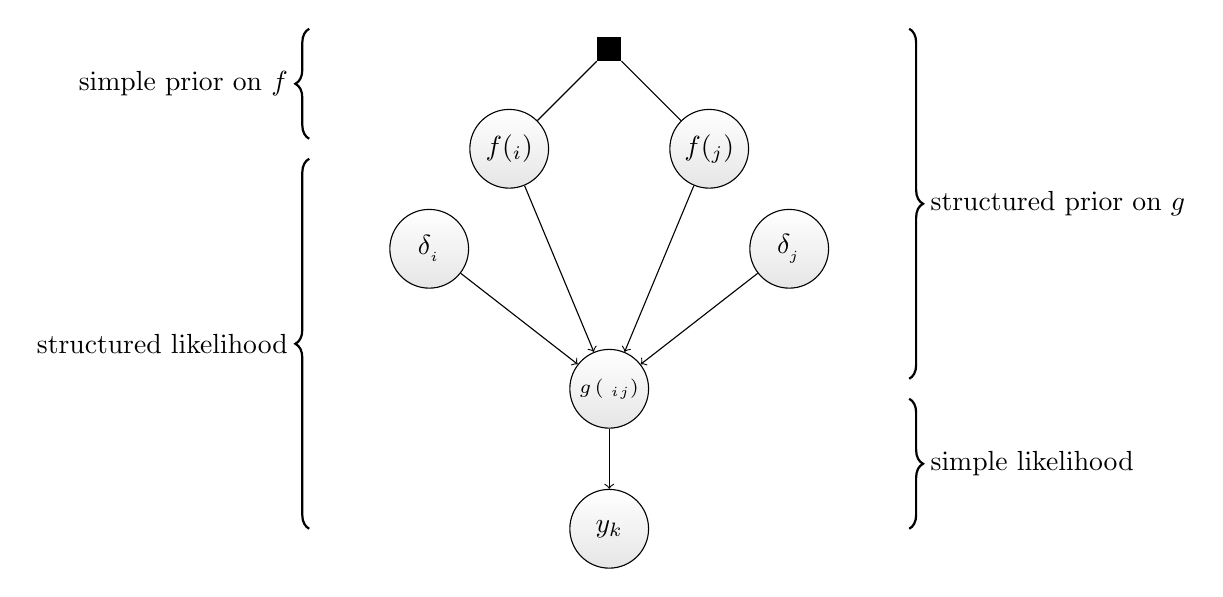
\begin{tikzpicture}
				\node at (2.5in,2.4in) [fill =black, rectangle,inner sep=0pt, minimum size = 0.3cm] (factor) {};
				\node at (2in,1.9in) [draw, circle,inner sep=0pt, minimum size = 1cm, top color=white, bottom color=black!10] (f_1) {$f(\x_i)$};
				\node at (3in,1.9in) [draw, circle,inner sep=0pt, minimum size = 1cm, top color=white, bottom color=black!10] (f_2) {$f(\x_j)$};
				\node at (1.6in,1.4in) [draw, circle,inner sep=0pt, minimum size = 1cm, top color=white, bottom color=black!10] (delta_2) {$\delta_{\x_i}$};	
				\node at (3.4in,1.4in) [draw, circle,inner sep=0pt, minimum size = 1cm, top color=white, bottom color=black!10] (delta_1) {$\delta_{\x_j}$};
				\node at (2.5in,0.7in) [draw, circle,inner sep=0pt, minimum size = 1cm, top color=white, bottom color=black!10] (g) {\scriptsize $g\left(\begin{matrix}\x_i\\\x_j\\\end{matrix}\right)$};
				\node at (2.5in,0in) [draw, circle,inner sep=0pt, minimum size = 1cm, top color=white, bottom color=black!10] (y) {$y_k$};
				\draw [->] (g) to (y);
				\draw  (factor) to (f_1);
				\draw (factor) to (f_2);
				\draw [->] (f_1) to (g);			
				\draw [->] (f_2) to (g);
				\draw [->] (delta_1) to (g);
				\draw [->] (delta_2) to (g);
				\draw [thick,decorate,decoration={brace,amplitude=5pt},] (1in,1.95in)  -- (1in,2.5in)
					node [black,midway,left=4pt] {simple prior on $f$};
				\draw [thick,decorate,decoration={brace,amplitude=5pt}] (1in,0in)  -- (1in,1.85in)
					node [black,midway,left=4pt] {structured likelihood};
				\draw [thick,decorate,decoration={brace,amplitude=5pt}] (4in,2.5in)  -- (4in,0.75in)
									node [black,midway,right=4pt] {structured prior on $g$};
				\draw [thick,decorate,decoration={brace,amplitude=5pt}] (4in,0.65in)  -- (4in,0in)
					node [black,midway,right=4pt] {simple likelihood};
			\end{tikzpicture}
	\end{center}
		\caption{Generative model underlying the preference learning framework. \emph{Left:} the original approach \citep{chu2005} considers the latent preference function $f$ as latent parameter, and the rest of the graphical model as a complex, structured likelihood. \emph{Right:} Our approach re-parametrises the problem in terms of $g$, and thus works with a simpler likelihood but with a more structured prior. The prior takes the form of a Gaussian Process with the preference judgement covariance function. \label{fig:graphical_model}}
\end{figure}


It is straightforward to show that the preference kernel, $k_{pref}$ is positive semi-definite. We can also see how $k_{pref}$ respects the anti-symmetry properties of preference learning, by computing the prior correlation between $g(\x_i,\x_j)$ and $g(\x_j,\x_i)$ as follows (assuming for brevity that $\mu_{pref}=0$):
 
 \begin{align}
 	\text{Corr}&(g(\x_i,\x_j),g(\x_j,\x_i)) = \frac{k_{pref}((\x_i,\x_j),(\x_j,\x_i))}{\sqrt{k_{pref}((\x_i,\x_j),(\x_i,\x_j))}\sqrt{k_{pref}((\x_j,\x_i),(\x_j,\x_i))}} \notag\\
 		&= \frac{k(\x_i,\x_j) + k(\x_j,\x_i) - k(\x_i,\x_i) - k(\x_j,\x_j)}{\sqrt{k(\x_i,\x_i) + k(\x_j,\x_j) - k(\x_i,\x_j) - k(\x_j,\x_i)}\sqrt{k(\x_j,\x_j) + k(\x_i,\x_i) - k(\x_j,\x_i) - k(\x_i,\x_j)}}\notag\\ &= -1\,.\notag
 \end{align}

That is, the value at $(\x_i,\x_j)$ is perfectly anti-correlated with the value at $(\x_j,\x_i)$ under the prior. From this fact it can be shown that all elements $g$ of the reproducing kernel Hilbert space (RKHS) corresponding to $k_{pref}$ have the property that $g(\x_i,\x_j) = -g(\x_j,\x_i)$. 

In summary, the combination of the likelihood in (\ref{eq:likelihood2})
with a GP prior based on this new preference kernel allows us
to transform the problem of learning preferences into a
GP binary classification problem on the space of features
$\mathcal{X}^2$. 
This means that state-of-the art methods
for GP binary classification, such as expectation propagation,
can be trivially used for addressing pairwise preference learning problems.
Furthermore, the simplified likelihood (\ref{eq:likelihood2})
allows us to easily implement complex methods 
such as the following multi-user approach.


